\documentclass[11pt,a4paper]{article}

\usepackage[utf8]{inputenc}
\usepackage[T1]{fontenc}
\usepackage[margin=2.5cm]{geometry}
\usepackage{amsmath,amssymb}
\usepackage{booktabs}
\usepackage{graphicx}
\graphicspath{{outputs/figures/}}

\usepackage{xcolor}
\usepackage{hyperref}
\usepackage{natbib}
\usepackage{setspace}
\usepackage{caption}
\usepackage{float}
\usepackage{array}
\usepackage{parskip}

\hypersetup{colorlinks=true,linkcolor=blue!60!black,
            citecolor=blue!60!black,urlcolor=blue!60!black}

\setlength{\parskip}{5pt}
\setlength{\parindent}{0pt}

\newcommand{\Fi}{F_i}
\newcommand{\nop}{\hat{n}}
\newcommand{\adag}{\hat{a}^\dagger}
\newcommand{\aop}{\hat{a}}
\newcommand{\rhohat}{\hat{\rho}}
\newcommand{\Lop}{\hat{L}}

\title{Targeted Dephasing as a Causal Handle on Local\\
       Occupation Loss in an Open Bose--Hubbard Chain}

\author{Kunal Bhatia\\
\small Independent Researcher\quad\texttt{kunal29bhatia@gmail.com}}

\date{March 2026\quad\textit{Preprint --- not peer reviewed}}

\begin{document}
\maketitle

\begin{abstract}
In an open one-dimensional Bose--Hubbard chain with Lindblad dephasing,
targeted additional dephasing at sites of high local occupation variance
produces more future local occupation loss than matched-budget random
targeting in the $J/U=0.30$--$0.40$ regime.
The effect is positive and robust at $J/U\in\{0.30,0.40\}$ across three
time horizons ($\tau\in\{1,2,3\}$) and two chain lengths ($L\in\{6,7\}$),
with bootstrap confidence intervals excluding zero at every tested point
in that range.
The lowest tested coupling ($J/U=0.12$) is uniformly negative, while
$J/U=0.20$ is transitional and size-sensitive.
The observed spatial response is more consistent with nonlocal
redistribution of occupation loss than with a purely local-instability
account.
All results are computed by exact Lindblad evolution in the
fixed-particle-number sector; no approximations are used.
\end{abstract}

\section{Introduction}
\label{sec:intro}

The one-dimensional Bose--Hubbard model is a standard setting for studying
the interplay of quantum tunnelling and on-site interactions in interacting
boson systems~\citep{fisher1989,jaksch1998}.
At zero temperature the model exhibits a quantum phase transition between a
superfluid phase (large $J/U$) and a Mott-insulating phase (small $J/U$),
controlled by the ratio of tunnelling amplitude~$J$ to on-site
interaction~$U$.
In the presence of dissipation---modelled here by local dephasing in the
Lindblad framework---the system is driven away from the ground state and
develops spatially heterogeneous fluctuation structure.

In classical lattice systems, local structural variables can serve as
causal handles: targeted perturbations at structurally selected sites
produce measurably different future outcomes from matched-budget
perturbations at random sites~\citep{woodward2003}.
Whether analogous causal handles exist in open quantum systems---where
dynamics are governed by a Lindblad master equation and the state is a
density matrix rather than a classical configuration---is an empirical
question that has received little direct attention.

This paper tests one specific instance.
Under uniform dephasing, sites in the Bose--Hubbard chain develop different
local occupation variances $\Fi = \langle\nop_i^2\rangle -
\langle\nop_i\rangle^2$, reflecting the degree of local number
fluctuation.
We ask whether selecting the highest-$\Fi$ sites for additional dephasing
produces a different pattern of future occupation loss than applying the
same total dephasing budget to randomly chosen sites.
The question is about the causal accessibility of future dynamical
outcomes through structurally targeted interventions, not about the
equilibrium phase diagram.

\section{Model and Methods}
\label{sec:methods}

\subsection{Bose--Hubbard Hamiltonian}

The Hamiltonian for a chain of $L$ sites with open boundary conditions is
\begin{equation}
\label{eq:ham}
\hat{H} = -J\sum_{i=1}^{L-1}\bigl(\adag_i\aop_{i+1} + \mathrm{h.c.}\bigr)
         + \frac{U}{2}\sum_{i=1}^{L}\nop_i(\nop_i - 1),
\end{equation}
where $J$ is the tunnelling amplitude, $U$ the on-site interaction,
$\nop_i = \adag_i\aop_i$, and the local Fock space is truncated at
$n_{\max}=3$ occupations per site.
The system is studied at half-filling ($N=\lfloor L/2\rfloor$ particles) in
the fixed-particle-number sector.
Open boundary conditions are used throughout, so that the local variance
field $\Fi$ can develop nontrivial spatial structure across the chain.

\subsection{Hilbert space}

The computation is restricted to the sector of exactly $N$ particles
distributed across $L$ sites, each with at most $n_{\max}=3$ occupations.
The dimension of this sector is $\binom{L+N-1}{N}$ reduced by the
$n_{\max}$ constraint; for $L=6$, $N=3$ the dimension is $D=56$, and for
$L=7$, $N=3$ it is $D=84$.
All operators are constructed as dense matrices in this basis.

\subsection{Lindblad dynamics}

The density matrix $\rhohat$ evolves under the Lindblad master equation
\begin{equation}
\label{eq:lindblad}
\frac{d\rhohat}{dt} = -i[\hat{H},\rhohat]
  + \sum_{i=1}^{L} \gamma_i \Bigl(
    \Lop_i\rhohat\Lop_i^\dagger
    - \tfrac{1}{2}\{\Lop_i^\dagger\Lop_i,\,\rhohat\}
  \Bigr),
\end{equation}
where $\Lop_i = \nop_i$ is a dephasing jump operator and $\gamma_i$ is
the dephasing rate at site~$i$.
Baseline dephasing is uniform: $\gamma_i = \gamma = 0.1$ for all sites.
Dephasing does not change $\langle\nop_i\rangle$ at the moment of
application; it decoheres number-state superpositions without injecting or
removing particles.

The Lindblad equation is converted to a superoperator acting on the
vectorised density matrix.
Time evolution is computed by the action of the matrix exponential on
the state vector, using \texttt{scipy.sparse.linalg.expm\_multiply}, which
avoids forming the full propagator and is the main computational
bottleneck.
No Trotter decomposition, stochastic unravelling, or other approximation
is used.

\subsection{Burn-in state}

The initial state is the ground state of $\hat{H}$, obtained by exact
diagonalisation.
This pure state is then evolved under uniform baseline dephasing for a
burn-in period $t_{\mathrm{burn}}=5.0$ (in units of $\hbar/U$).
The resulting mixed state $\rhohat_{\mathrm{burn}}$ serves as the starting
point for all interventions within a given condition.
The burn-in ensures that the state has developed spatially heterogeneous
fluctuation structure under dissipation before any intervention is applied.

\subsection{Handle definition}

The handle variable is the local occupation variance
\begin{equation}
\label{eq:Fi}
\Fi = \langle\nop_i^2\rangle - \langle\nop_i\rangle^2,
\end{equation}
evaluated on the post-burn-in state $\rhohat_{\mathrm{burn}}$.
This quantity identifies sites with larger number fluctuations.
Under open boundary conditions, $\Fi$ is typically largest at the central
sites of the chain, where the tunnelling network is most connected, and
smallest at the edges.
The top-$k$ sites by $\Fi$ ($k=\lceil L/3\rceil$) are selected for
intervention.
The selected set is fixed by the post-burn-in state and is therefore
deterministic within each condition.

\subsection{Intervention protocol}

The \textbf{targeted intervention} applies additional dephasing
$\gamma_{\mathrm{extra}}=0.5$ at the selected high-$\Fi$ sites, keeping
all other sites at the baseline rate $\gamma$.
The \textbf{random control} applies the same total extra budget
($k\times\gamma_{\mathrm{extra}}$) to $k$ randomly chosen sites.
In both cases the total dissipative budget is identical.
Because $\Lop_i=\nop_i$ commutes with the total number operator,
$\langle\nop_i\rangle$ is unchanged at the moment of intervention by
construction; the occupation profile is held fixed.

The targeted intervention is deterministic: for a given condition, the
post-burn-in state and the selected sites are the same, so the targeted
evolution is computed once per $(\text{condition},\tau)$ pair.
Only the random arm varies across trials.

\subsection{Target}

The primary target is local future occupation loss at the intervention
sites:
\begin{equation}
\label{eq:target}
\mathcal{L}_{\mathrm{local}}(\tau) =
  \sum_{i\in\mathcal{S}}
  \max\bigl(0,\;\langle\nop_i\rangle_t - \langle\nop_i\rangle_{t+\tau}\bigr),
\end{equation}
where $\mathcal{S}$ is the set of selected sites and $\tau$ is the
measurement horizon.

\subsection{Design and statistical analysis}

Four tunnelling-to-interaction ratios $J/U\in\{0.12,0.20,0.30,0.40\}$ are
tested, spanning from deep Mott-like to intermediate superfluid-like
regimes.
Three horizons $\tau\in\{1,2,3\}$ and two chain lengths $L\in\{6,7\}$
are used.
For each condition, $N_{\mathrm{trials}}=100$ independent random-site draws
are compared against the single targeted intervention.
The test statistic is the mean difference in $\mathcal{L}_{\mathrm{local}}$
between targeted and random interventions.
A 95\% bootstrap confidence interval (1000 resamples, trial-level
resampling) is constructed for each condition.
The decision rule is that a condition passes if the lower bound of the
95\% CI exceeds zero.

\section{Results}
\label{sec:results}

\subsection{Main result at $L=6$}

Table~\ref{tab:main} reports the local-loss difference for all conditions
at $L=6$.
At $L=6$, the targeted intervention produces more local occupation loss
than the random control throughout $J/U\in\{0.20,0.30,0.40\}$, with all
confidence intervals in that range excluding zero, while the broader
cross-size regime map (Section~\ref{sec:regime}) shows that $J/U=0.20$ is
transitional.
The lowest tested coupling $J/U=0.12$ is uniformly negative: the targeted
intervention produces \emph{less} local loss than matched-budget random
targeting at all three horizons.

\begin{table}[H]
\centering
\caption{Local-loss difference (targeted $-$ random) at $L=6$,
$N_{\mathrm{trials}}=100$ per condition.
Format: mean $[\text{95\% CI}]$.
$J/U=0.12$ is uniformly negative (boundary regime).}
\label{tab:main}
\begin{tabular}{l ccc}
\toprule
$J/U$ & $\tau=1$ & $\tau=2$ & $\tau=3$ \\
\midrule
0.12 & $-0.002$ $[-0.002,\,-0.001]$ & $-0.002$ $[-0.003,\,-0.002]$ & $-0.002$ $[-0.003,\,-0.001]$ \\
0.20 & $0.001$ $[0.000,\,0.001]$ & $0.006$ $[0.005,\,0.007]$ & $0.011$ $[0.009,\,0.012]$ \\
0.30 & $0.013$ $[0.012,\,0.014]$ & $0.029$ $[0.027,\,0.031]$ & $0.040$ $[0.036,\,0.043]$ \\
0.40 & $0.019$ $[0.017,\,0.021]$ & $0.040$ $[0.036,\,0.043]$ & $0.047$ $[0.042,\,0.051]$ \\
\bottomrule
\end{tabular}
\end{table}

The effect increases with $J/U$ from the negative boundary at 0.12
through a transitional regime at 0.20 and into the robust positive
pocket at 0.30--0.40.
The magnitude of the positive difference also increases with the time
horizon~$\tau$, consistent with a cumulative dynamical effect rather than a
transient perturbation.

\begin{figure}[H]
\centering
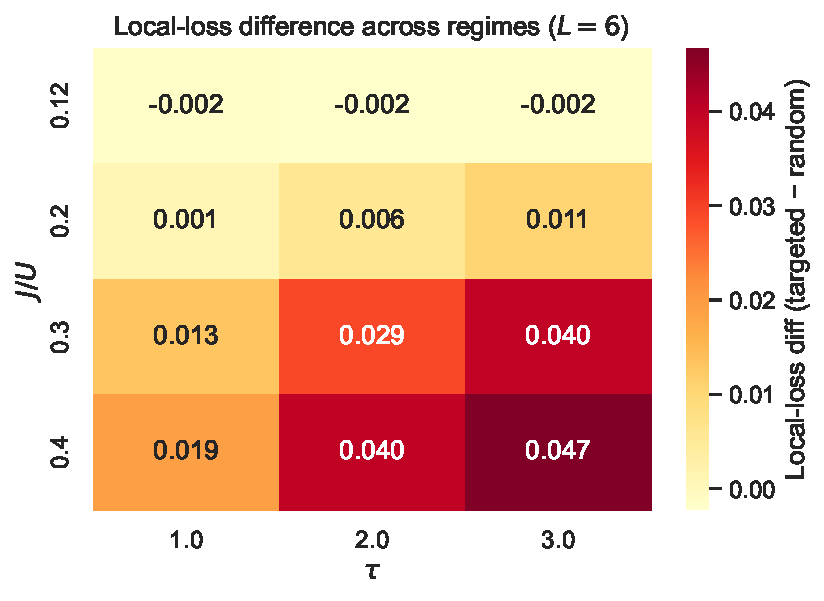
\includegraphics[width=0.85\linewidth]{fig1_main_heatmap.pdf}
\caption{Local-loss difference across $J/U$ and $\tau$ at $L=6$.
The handle effect is positive in the intermediate and stronger coupling
regime and absent or reversed at the lowest tested coupling.}
\label{fig:main_heatmap}
\end{figure}

\subsection{Robustness across chain length}

Table~\ref{tab:robust} compares pooled results at $J/U\in\{0.30,0.40\}$
for $L=6$ and $L=7$.
Both couplings pass at both chain lengths with confidence intervals
excluding zero, confirming that the positive pocket is not a single-size
artefact.

The intermediate coupling $J/U=0.20$ is size-sensitive: it passes at $L=6$
across all horizons but is not robust at $L=7$, where only the longest
horizon ($\tau=3$) produces a positive CI.
This places $J/U=0.20$ in a transitional regime whose handle effectiveness
depends on system size.

\begin{table}[H]
\centering
\caption{Pooled local-loss difference for $L=6$ and $L=7$ at
$J/U=0.30$ and $0.40$.
Format: mean $[\text{95\% CI}]$, pooling trial-level differences across
$\tau\in\{1,2,3\}$.}
\label{tab:robust}
\begin{tabular}{l cc}
\toprule
Condition & $L=6$ & $L=7$ \\
\midrule
$J/U=0.30$ & $0.027$ $[0.025,\,0.029]$ & $0.030$ $[0.028,\,0.032]$ \\
$J/U=0.40$ & $0.035$ $[0.033,\,0.038]$ & $0.047$ $[0.044,\,0.050]$ \\
\bottomrule
\end{tabular}
\end{table}

\begin{figure}[H]
\centering
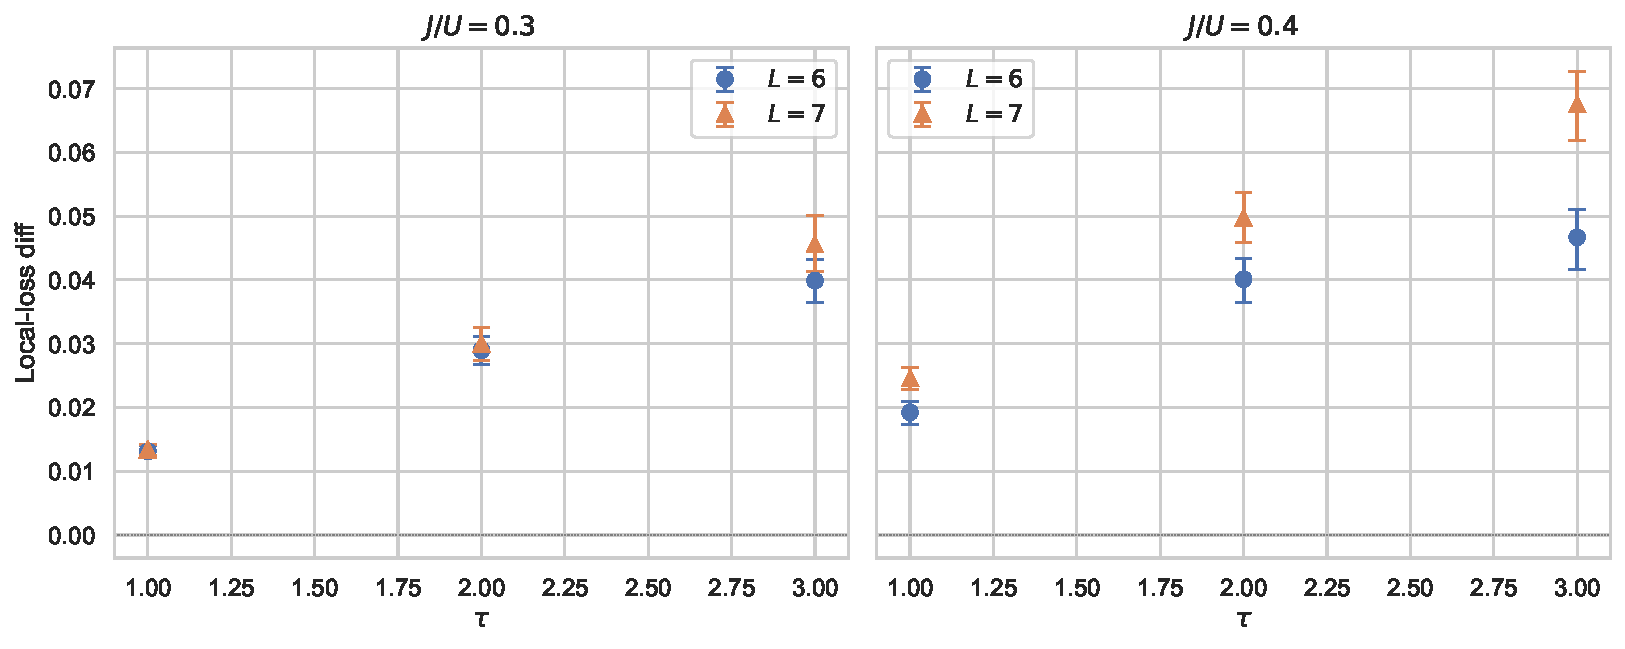
\includegraphics[width=0.85\linewidth]{fig2_robustness.pdf}
\caption{Local-loss difference at $J/U=0.30$ and $0.40$ for
$L=6$ and $L=7$. Error bars are 95\% bootstrap CIs.
The positive pocket persists across both chain lengths.}
\label{fig:robustness}
\end{figure}

\subsection{Regime map}
\label{sec:regime}

The results define three regimes within the tested parameter range:

\textbf{Negative regime} ($J/U=0.12$):
The targeted intervention produces less local loss than random targeting at
both chain lengths and all horizons.
In this deep Mott-like regime the occupation-variance handle does not
identify causally effective sites.

\textbf{Transitional regime} ($J/U=0.20$):
Positive at $L=6$ but not robust at $L=7$.
The handle begins to function but its effectiveness is size-dependent.

\textbf{Positive pocket} ($J/U\in\{0.30,0.40\}$):
The handle is consistently positive across both chain lengths and all
horizons.
This is the regime where the occupation-variance selector reliably
identifies sites whose perturbation produces excess local loss.

The existence of a negative boundary regime and a transitional zone is
itself informative: the handle is not a generic property of the dephasing
operator but depends on the dynamical regime of the system.

\subsection{Spatial response pattern}

Figure~\ref{fig:mechanism} shows the site-resolved occupation change under
targeted versus random intervention at $J/U=0.30$, $L=6$, $\tau=2$.
The bars show mean site-resolved occupation change under the deterministic
targeted intervention and averaged across the 40 matched-budget random
interventions.

The observed pattern is consistent with a nonlocal, redistributive
response.
Under targeted intervention, the selected sites (shaded) tend to show
\emph{less} negative occupation change than under random intervention:
selected-site loss is reduced relative to random targeting.
At the same time, non-selected sites show increased occupation loss under
targeted intervention.
The net effect is that the intervention changes the spatial pattern of
occupation change across the chain rather than simply amplifying loss at
the targeted sites themselves.

This is the opposite of what a purely local-instability mechanism would
predict, in which extra dephasing at a high-$\Fi$ site would increase loss
specifically at that site.
The data are more consistent with a picture in which perturbing high-$\Fi$
sites alters the subsequent spatial distribution of occupation change
across the chain.

\begin{figure}[H]
\centering
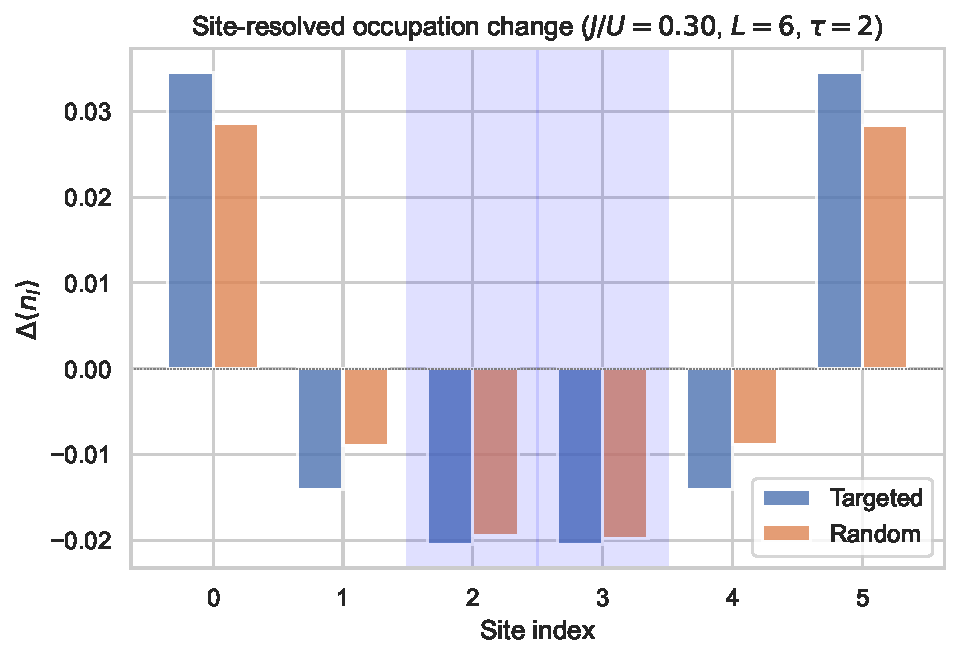
\includegraphics[width=0.85\linewidth]{fig3_mechanism.pdf}
\caption{Mean site-resolved occupation change under the targeted
intervention and across matched-budget random interventions
($J/U=0.30$, $L=6$, $\tau=2$).
Negative values correspond to occupation loss.
Shaded bands mark selected sites.
The spatial response is consistent with nonlocal redistribution.}
\label{fig:mechanism}
\end{figure}

\section{Discussion}
\label{sec:disc}

\paragraph{Summary.}
In an open Bose--Hubbard chain, sites of high local occupation variance
serve as causal handles in the intermediate and stronger coupling regime:
targeting them with additional dephasing produces more local future
occupation loss than matched-budget random targeting at
$J/U\in\{0.30,0.40\}$, robustly across both tested chain lengths and all
tested horizons.
The effect is absent or reversed at the lowest tested coupling
($J/U=0.12$) and transitional at $J/U=0.20$.

\paragraph{Mechanism.}
The site-resolved response is more consistent with nonlocal redistribution
than with local instability.
Perturbing high-$\Fi$ sites is associated with a redistribution of
subsequent occupation change across the chain.
A complete mechanistic account is beyond the scope of the present analysis.

\paragraph{What is not claimed.}
We do not claim that high-$\Fi$ targeting is optimal among all possible
intervention strategies, that the effect extends to all coupling regimes
(it does not hold at $J/U=0.12$ and is only transitional at $J/U=0.20$),
that the mechanism generalises to other quantum systems or larger chains,
or that the occupation-variance handle corresponds to any equilibrium
observable.

\paragraph{Scope and limitations.}
The causal-handle effect is regime- and size-dependent in the present
design, with the clearest fully robust support in the
$J/U=0.30$--$0.40$ regime.
The Hilbert-space dimension of the fixed-$N$ sector grows combinatorially
with $L$ and $n_{\max}$, limiting exact Lindblad evolution to small chains.
The tested range ($L\leq7$, $n_{\max}=3$) establishes the effect in the
positive pocket but does not access the thermodynamic limit.
Whether the positive pocket persists, broadens, or shifts at larger system
sizes is an open question requiring approximate methods such as
matrix-product-state Lindblad evolution.

\section*{Data and Code Availability}

All simulations, figures, and tables are generated by running
\texttt{python bh.py} in the accompanying package.
The build script \texttt{build.sh} runs the simulation and compiles this
manuscript from the generated outputs.
All parameters and random seeds are defined in the source code.

\bibliographystyle{plainnat}
\begin{thebibliography}{9}

\bibitem[Fisher et~al.(1989)]{fisher1989}
Fisher, M.\,P.\,A., Weichman, P.\,B., Grinstein, G., and Fisher, D.\,S.
(1989).
Boson localization and the superfluid-insulator transition.
\textit{Phys.\ Rev.\ B}, 40(1):546--570.

\bibitem[Jaksch et~al.(1998)]{jaksch1998}
Jaksch, D., Bruder, C., Cirac, J.\,I., Gardiner, C.\,W., and Zoller, P.\
(1998).
Cold bosonic atoms in optical lattices.
\textit{Phys.\ Rev.\ Lett.}, 81(15):3108--3111.

\bibitem[Woodward(2003)]{woodward2003}
Woodward, J.\ (2003).
\textit{Making Things Happen: A Theory of Causal Explanation}.
Oxford University Press.

\end{thebibliography}

\end{document}